%        File: LitReview.tex
%     Created: Thu Oct 05 09:00 AM 2017 E
% Last Change: Thu Oct 05 09:00 AM 2017 E
%
% arara: pdflatex: {options: "-draftmode"}
% arara: biber
% arara: pdflatex: {options: "-draftmode"}
% arara: pdflatex: {options: "-file-line-error-style"}
\documentclass[MilwayThesis]{subfiles}
\setcounter{chapter}{2}
\begin{document}
In this chapter I will review several previous analyses of adjectival resultatives and the parametric variation associated with them.
I will evaluate the anlyses against two desiderata.
First, I will evaluate whether the variation, as analyzed, is learnable.
Second, I will evaluate whether the analysis comports with the theoretical principles of the minimalist program.
Before reviewing the analyses, however, I will make these desiderata explicit and justify them.

\section{Desiderata for an analysis of resultatives}

\subsection{Desideratum 1: Learnability}
Most of the analyses of the structure of adjectival resultatives are packaged with an account of the associated parametric variation, and it is a truism that any aspect of a language that varies from speaker to speaker must be acquirable from the primary linguistic data.
While few address directly address the acquisition of parametric variation, any analysis of variation makes implicit claims about acquistion.
Frequently, when discussing parametric variation, the claims about acquisition are left implicit, as the acquisition task is assumed to be trivial.
The nature of adjectival resultatives, however, is such that we must make those acquisition claims explicit.
To explain why, I will be comparing the resultative parameter to the V-to-T parameter.

Analyses of the V-to-T parameter do not need to address learnability because the ``parameter setting'' is directly learnable from the primary linguistic data.
It is directly learnable because the overt forms of (\textit{e.g.}) polar questions differ depending on the parameter setting.
In a language with V-to-T movement such as German, the language learner will observe that lexical verbs undergo inversion for polar questions, while in a language without V-to-T movement such as English, the learner will observe that lexical verbs do not invert for questions.
\ex. V-to-T movement (German)
\ag. Trinken sie Kaffee?\\
Drink.3plPres they Coffee\\
``Do they drink coffee?''
\bg.* Tun sie Kaffee trinken?\\
do they coffee drink\\

\ex. *V-to-T Movement (English)
\a.* Drink they coffee?
\b. Do they drink coffee?

The form of polar questions, then, can be positive evidence for a particlar setting of a parameter.
Since we can find direct positive evidence for a parameter setting, the task of the analyst/theoretician, then is merely to formalize the parameter is a way that is consistent with the broader theory.
\textcite{chomsky1995minimalist}, for instance, formalizes the V-to-T parameter in terms of feature strength, while \textcite{lasnik1999verbal} formalizes it in terms of the presence/absence of inflectional features on lexical verbs.
Neither, however, needs to explicitly describes how their parameter is set, but it can assumed that a certain setting is the default, and the other setting can be deduced from (\textit{e.g.}) the form of polar questions in the language.

Resultatives, on the other hand, are not directly learnable for two reasons.
The first reason is that, on the surface, resultatives, which are parameterized, are indistinguishable from depictives, which appear to be universal.
The two construction types are indistinguishable in the sense that both correspond to the string template in \Next (modulo independent word order variation).
\ex. \textsc{Subj} V \textsc{Obj} Adj.

This indistinguishability is evident in the fact that one can construct examples which are truly ambiguous between resultative and depictive readings, as in \Next.
\ex. 
\a. He fried the fish dry.
\a. $\approx$ He fried the fish once it was dry. (\textbf{Depictive})
\b. $\approx$ He fried the fish until it was dry. (\textbf{Resultative})
\z.
\b. She painted the barn red.
\a. $\approx$ The barn is red in her painting. (\textbf{Depictive})
\b. $\approx$ She applied a coat of red paint to the door. (\textbf{Resultative})
\z.

Assuming a child acquiring either French or English encounters sentences with the form of \LLast in their PLD, there is no obvious way for the child to determine whether a given secondary predicate is to be interpreted depictively or resultatively.

An empiricist might object, arguing that the ambiguous examples above are highly constructed, and would easily by disambiguated in context.
They would insist that the learner would infer a positive setting of the resultative parameter from the use of a secondary predication construction in the presence of a resultative event.
So, an English learner, but not a French learner, might be exposed to the context-sentence pairing in \Next.
\ex. 
\a.[\textbf{Context:} ] A woman is methodically hammering a lump of metal.
A parent draws their child's attention to the hammering event and utters:
\b.[\textbf{A:}] She's hammering the metal flat.

Even this, however, is not fully unambiguous.
While it certainly couldn't be interpreted as a depictive, \textit{flat} could plausibly be interpreted by a child as a manner adverb, modifying \textit{hammering}.
Such unavoidable ambiguity would make it difficult to employ any sort of semantic bootstrapping in the acquisition of the resultative parameter.\footnote{
	This line of argumentation is inspired by \textcite{gleitman1990structural,carey1985constraints,quine1960word} 
}

The second problem comes from the fact that both English-type and French-type languages can express resultative semantics periphrastically as in \Next.
\ex. \textbf{Periphrastic Resultatives}
\ag. Elle a aplati le m\'etal en le martelant\\
She has flattened the metal in the hammering\\
\b. She flattened the metal by hammering.

The resultative parameter, then, is a one-or-both parameter, meaning the presence of periphrastic resultatives in the PLD cannot be conclusive evidence of either setting of the resultative parameter.
The V-to-T parameter, in contrast, is an either/or parameter, meaning \textit{e.g.} the presence of \textit{do}-support can be taken as evidence of a negative setting.

Since there is no direct way to determine from the primary linguistic data whether a language allows or disallows resultatives, we can reject any analysis of resultatives that requires the parameter to be directly set based on primary linguistic data..
Rather, the setting of the resultative parameter must be derived from the setting of a parameter which can be directly acquired.

\subsection{Desideratum 2: Theoretical consistency}
The second quality an analysis of resultatives should have is consistency with the broader theory of grammar.
While this is a requirement of all analyses of grammatical phenomena, I will outline the subset of minimalist hypotheses that I will use to evaluate proposed analyses of adjectival resultatives.
First, I will review what is called the Uniformity of Theta Hypothesis (UTAH) which gives us a baseline for our theory of $\Theta$-role assignment.
Second, I will look at the Borer-Chomsky Conjecture, which is the minimalist hypothesis which will guide our theory of variation.
Each of these will be discussed with reference to a particular property of adjectival resultatives.

The canonical formulation of UTAH is that of \textcite{baker1988incorporation} working in pre-minimalist Principles and Parameters framework, given below in \Next.
\ex. \textbf{The Uniformity of Theta Hypothesis (UTAH)}\\
Identical thematic relationships between items are represented by identical structural relationships between those items at the level of D-structure. \parencite[46]{baker1988incorporation}

While I will be assuming something of this sort in my discussion, the reference to D-structure, which was eliminated in the minimalist program, renders Baker's hypothesis unusable as it stands.
I propose the following more precise formulation of UTAH:
\ex. \textbf{Minimal UTAH}\\
If a thematic relation $f$ holds between items X and Y in distinct expressions S$_1$ and S$_2$, then there is a single structural relation $g$ that also holds between X and Y in both S$_1$ and S$_2$.

To understand what this means, consider the following sentence pairs:
\ex. \label{ex:broke-bottle}
\a. Sara broke the bottle.
\b. The bottle broke.

\ex. \label{ex:katie-ran}
\a. Katie ran.
\b. Katie ran a kilometre.

The pair in \ref{ex:broke-bottle} represents a single thematic relation between \textit{broke} and \textit{the bottle}.
UTAH says that there must be a structural relation that holds between \textit{broke} and \textit{the bottle} in both sentences.
Similarly, in \ref{ex:katie-ran}, there is a single thematic relation between \textit{Katie} and \textit{ran}, which means there must be a single corresponding structural relation between the two.
Any structural analysis of these sentences that violates Minimal UTAH, then, can be rejected on theoretical grounds.

Consider, for instance, three possible structural analyses of the pair in \ref{ex:broke-bottle}.
In the first analysis, represented in \Next, \textit{the bottle} is base generated in its surface position, which is different in the two sentences.
\ex. \textbf{The surface analysis}
\a. \textit{Sara broke the bottle.}\\
\begin{forest}
  nice empty nodes,sn edges,baseline
  [TP
    [DP[Sara,roof]]
    [
      [T]
      [VP
        [V\\broke,align=center]
        [DP[the bottle,roof]]
      ]
    ]
  ]
\end{forest}
\b. \textit{The bottle broke.}\\
\begin{forest}
  nice empty nodes,sn edges,baseline
  [TP
    [DP[the bottle,roof,name=subj]]
    [
      [T]
      [VP[broke,roof]]
    ]
  ]
\end{forest}

In this analysis, there is no single structural relation between \textit{broke} and \textit{the bottle}, corresponding to the single thematic relation.
This analysis, then, violates Minimal UTAH, and can therefore be rejected.

In the second analysis, represented in \Next, \textit{the bottle} originates in [Comp V] and moves to subject position in the intransitive situation.
\ex. \textbf{The movement analysis}
\a. \textit{Sara broke the bottle.}\\
\begin{forest}
  nice empty nodes,sn edges,baseline
  [TP
    [DP[Sara,roof]]
    [
      [T]
      [VP
        [V\\broke,align=center]
        [DP[the bottle,roof]]
      ]
    ]
  ]
\end{forest}
\b. \textit{The bottle broke.}\\
\begin{forest}
  nice empty nodes,sn edges,baseline
  [TP
    [DP[the bottle,roof,name=subj]]
    [
      [T]
      [VP
        [V\\broke,align=center]
        [DP[the bottle,roof,name=theme]]
      ]
    ]
  ]
  \draw[->] (theme) to[out=south west, in=south] (subj);
\end{forest}

In this analysis the single thematic relation between \textit{broke} and \textit{the bottle} corresponds to a single structural relation between the two.
While UTAH considerations clearly lead us to prefer the movement analysis over the surface analysis, such considerations are far from decisive evidence in favour of the movement analysis, as it is not the only possible analysis that complies with UTAH.

Another UTAH-compliant account, which I will call the layering analysis, is represented in \Next.
This type of analysis is proposed by \textcite{borer2005normal,ramchand2008verb}.

\ex. \textbf{The layering analysis}
\a. \textit{Sara broke the bottle}
\begin{forest}
  nice empty nodes,sn edges,baseline
  [vP
    [DP[Sara,roof]]
    [
      [v$_{EA}$]
      [vP
        [DP[the bottle,roof]]
        [
          [v$_{IA}$]
	  [V\\broke,align=center]
        ]
      ]
    ]
  ]
\end{forest}
\b. \textit{The bottle broke.}
\begin{forest}
  nice empty nodes,sn edges,baseline
  [vP
    [DP[the bottle,roof]]
    [
      [v$_{IA}$]
      [V\\broke,align=center]
    ]
  ]
\end{forest}

In this analysis, as in the movement analysis, the thematic relation between \textit{broke} and \textit{the bottle} is represented by a single structural relation between the two.
This means that this analysis also satisfies Minimal UTAH, and therefore cannot be rejected immediately.

UTAH is relevant to adjectival resultatives considering the pattern of thematic relations in \Next.
\ex.
\a. Jackie hammered the metal flat.
\b. Jackie hammered the metal.
\b. Jackie made the metal flat.

There is a single $\Theta$ relation that holds between \textit{hammered} and \textit{the metal} in both \Last[a] and \Last[b], and there is a single $\Theta$ relation that holds between \textit{the metal} and \textit{flat} in  both \Last[a] and \Last[c]. 
Therefore, there should be a single structural relation corresponding to each of those $\Theta$ relations, and any analysis that does not meet this criterion will be rejected.

It could be noted that while a particular entailment pattern clearly and robustly holds of \Last (\Last[a] entails both \Last[b] and \Last[c]), the same cannot be said for all versions of adjectival resultatives.
Consider, for instance, \Next the English version of Kratzer's (\citeyear{kratzer2004building}) central example.
\ex. 
\a. We drank the teapot dry.\\
(\textit{cf.} \textit{Wir haben die Teekanne leer getrunken})
\b.?\# We drank the teapot.
\b. We made the teapot dry. 

While \Last[a] does clearly and robustly entail \Last[c], we cannot say the same about \Last[a] and \Last[b], as it is generally judged as highly coerced.
Presented with this pattern, we might argue that UTAH considerations are only informative regarding the structural relationship between the object and the adjective of resultatives like \Last[a].
The pattern in \Last does not, however, negate the pattern in \LLast, which suggested that the resultative object is $\Theta$-marked by its verb as well as its adjective.
We could propose that there are, in fact, atleast two distinct structures for resultatives: one corresponding to cases like \LLast, and another corresponding to cases like \Last.
To my knowledge, however, there is no corroborating evidence for any structural difference between \LLast[a] and \Last[a], and, absent any such evidence, we ought to assume they have the same structure.
Given this, we must decide which type of resultative we take a ``prototypical''.
If \Last[a] is our prototype, then we would assume that the resultative object is not $\Theta$-marked by its verb and we would have to explain why the object of \LLast[a] seems to be $\Theta$-marked by its verb.
There are, in my mind, two possible ways to explain this: we could either retain a single structure for resultatives and argue that \textit{the metal} is really not $\Theta$-marked by \textit{hammer} in \textit{hammer the metal flat}, or we could propose multiple structures for resultatives depending on their $\Theta$-marking properties.

The first line of argument means that we would need to propose at least one situation in which a thematic relation is established without explicit $\Theta$-marking, that is, extragrammatically.
This means we would be proposing an exception to UTAH, meaning we would need to explain why resultatives are exceptional.
If resultatives are not truly exceptional, then they are the norm and UTAH-compliant cases are the exceptions, meaning we would have to reject UTAH wholesale.
Neither of these are theoretically attractive options, so I will not pursue them any further here.

The second line of argument -- that there are multiple structures associated with resultatives -- violates the scientific principle of theoretical parsimony.
This means that, while we can't reject it outright, we should hold it as a last resort.

So, assuming Kratzer's example to be our prototype leads us to undesirable results.
Assuming \textit{hammer the metal flat} to be the prototype, I argue, does not lead us to any undesirable conclusions, though it does present some puzzles.
As in the discussion above, assuming one type of resultative to be prototypical means explaining the eccentricities in the non-prototypical version;
that is, we must explain the apparent lack of $\Theta$-marking in Kratzer's example.
While I cannot offer a full explanation, I will suggest that such an explanation will depend of a fuller understanding of the complex dynamics of coercion.



In addition to UTAH considerations, I will evaluate whether the theory of variation attached to a given analysis is formulable in the minimalist model of grammar.
This model of the grammar is composed of four parts:
	a lexicon containing the atoms from which complex expressions are built;
	merge, the simplest combinatorial operation for constructing complex expressions; 
	and two interfaces, points at which a constructed expression is transferred to language external modules for either externalization (the sensorimotor (SM) interface/module), or interpretation (the conceptual-intentional (CI) interface/module).
In this portion I will argue for what is known as the Lexical Parameterization Hypothesis (LPH) that the lexicon is the only component of grammar that can be the locus of parametric syntactic variation.\footnote{ 
	The earliest version of this hypothesis, formulated by Hagit Borer in the following way:
	\begin{quote}
		In this study we will propose a model of parameters which restricts the availability of variation to the possibilities which are offered by one single component: the inflectional component. \parencite[3]{borer1984parametric}
	\end{quote}
	Borer, however defines \textit{inflectional} in such a way that later work reformulates her proposal as restricting variation to the lexicon.
	See, for instance, an early version of the hypothesis by \textcite{manzini1987parameters} in ($i$) which they attribute to \textcite{borer1984parametric}
	\ex.[($i$)]
	\begin{minipage}[t]{\textwidth - 4em}
		\textbf{Lexical Parameterization Hypothesis}\\
		Values of a parameter are associated not with particular grammars but with particular lexical items. \parencite[424]{manzini1987parameters}
	\end{minipage}

} 
I will do so first by a positive argument -- that the lexicon is a natural place to locate variation -- then by a negative argument -- that neither merge, nor the interfaces can be parameterized.

The notion that lexicons vary may seem trivial, but it is worth describing if only to distinguish the grammatically relevant variation from the grammatically irrelevant variation.
This dichotomy roughly seems to follow the functional/lexical distinction.
Variation between two speakers with respect to lexical vocabulary can be fairly profound without necessarily meaning that the speakers are speaking a different language.
The variation relevant to this thesis, however, is the kind which leads to systemic differences between grammars.
For instance, consider the link between verbal agreement and pro-drop.
Synthesizing a broad set of empirical studies, \textcite{huang1984distribution} observes that only those languages with rich agreement morphology (\textit{e.g.}, Italian and Spanish) or no agreement morphology (\textit{e.g.}, Mandarin and Japanese) allow subject pro-drop.
If we take the richness of agreement to be a lexical parameter, then we have evidence that lexical variation can lead to systemic variation between grammars, and it is reasonable to consider agreement to be a lexical property.

The English verbal system provides us with good reason to consider richness of agreement to be lexical.
In English, main verbs and modals differ with respect to their agreement, with main verbs showing impoverished agreement and modals showing no agreement.
Regardless of the details of the analysis of this variation, there must be some lexical property that determines whether or not a verbal element surfaces with agreement morphology.
Since agreement morphology can be a variable lexical property within a language, it is reasonable to assume that it can be a variable lexical property accross languages.
Following this line of reasoning, and assuming that the pro-drop parameter is correlated with agreement morphology, the pro-drop parameter can be reduced to a lexical parameter.

Having shown that there can be significant grammatical effects from lexical variation, I will now argue that the remaining components of the grammar (merge, the two interfaces) are ill-suited to variation.

Merge is the simplest component to eliminate from consideration of the locus of variation due to its simplicity.
As defined in \Next, it iss the simplest possible operation for generating hierarchical structures: binary set formation.
\ex. Merge$(\alpha, \beta) = \{ \alpha, \beta\}$

In order to attribute crosslinguistic variation to merge, we would need to introduce complexity to it, and it would no longer be maximally simple.

It is worth noting, however, that merge, as defined in \Last, is not \textit{the} simplest possible combinatory operation, but the simplest one capable of generating hierachical structures.
\textcite{hornstein2009theory}, for instance, proposes a concatenative version of merge.
\ex. Merge$^\prime(\alpha, \beta) = \alpha^\frown\beta$

Assuming concatenation is as simple as set-formation, it is still not able to form hierachical structures without further complication.
This is because concatenation, unlike binary set-formation, is associative.
\ex. Merge$^\prime($ Merge$^\prime(\alpha, \beta), \gamma)$\\
$= (\alpha^\frown\beta)^\frown\gamma$\\
$= \alpha^\frown\beta^\frown\gamma$\\
$= \alpha^\frown(\beta^\frown\gamma)$\\
$= $Merge$^\prime(\alpha, $ Merge$^\prime(\beta, \gamma))$

Since concatenative merge forms essentially flat structures, it is ill-suited to construct linguistic expressions which appear to be fundamentally hierarchical in nature.
So, while there are other possible combinatory operations which are as simple as merge, there don't seem to be any which are able to capture the fact that linguistic expressions are hierarchically structured objects.
Therefore, any variation in merge can only come from complicating the operation.

The interfaces cannot be parameterized for reasons having to do with the logical problem of language acquisition.
If we take a grammar to be a mapping between form and meaning then we can represent it as a function.
As a function it will have a domain (meanings), a range (forms), and an intension (the grammar).
From these three properties we will be able to generate an extension of the function.
The language acquisition process, then, will be a process of inferring the function from a finite and arbitrary subset of its extension.
Such an inference 

Consider the following analogy to quadratic functions.
Suppose we model a particular I-function as the quadratic function in \Next, and the E-function it generates is it graph in \NNext.
\ex. I-Language$_x$\\
$y = 2x^2 + 4x-1$

\ex. E-Language$_x$\\
\includegraphics[width=0.7\textwidth]{quadplot-axis}

The task of acquisition, then, is analogous to fitting points to a polynomial function, and the question at hand is how many aspects of the polynomial must we know in order to properly define it given its graph.
Supposing we are not given the coefficients but rather merely a general quadratic function as in \Next and the graph in \Last.
\ex. $y = ax^2 + bx + c$

It would be trivial to compute the values of the coefficients from the information given.
Similarly, if we are given the fully specified function and its graph with an unspecified x-axis as in \Next
\ex. E-language$_x$\\ 
\includegraphics[width=0.7\textwidth]{quadplot-y-only}

We would be able to find the x-axis that makes the graph correspond to the function, and similar logic would follow if only the y-axis were missing.

It seems, then, that any single aspect of the function is missing, we would be able to reconstruct it based on the remaining information.
However, if we remove any two aspects, we will be unable to reconstruct either of them. 
Consider the fitting task if we are given a parabola with only a y-axis as in \Last.
Our task them is to determine the x-axis and the coefficients that are consistent with the parabola and y-axis, which would be an impossible task given that there would be an infinite number of consistent axis-coefficient pairs.

If we accept this as a reasonable analogy for language acquisition, then we are forced to only allow a single locus of variation.
Since I have already shown that lexical variation exists and can affect the grammar as a whole.
What follows from this is what is known as the Borer-Chomsky conjecture.
\ex. \textbf{The Borer-Chomsky Conjecture} \parencite{baker2008microparameter}\\
All parameters of variation are attributable to differences in the features of particular items (e.g., the functional heads) in the lexicon.

So any account of the resultative parameter must be explainable in lexical terms in order to be consistent with the Borer-Chomsky Conjecture.

The two theoretical principles discussed above will allow me to evaluate the previously proposed analyses of resultatives.
UTAH considerations will determine if a given structural analysis is tenable in minimalist syntax.
The Borer-Chomsky conjecture, on the other hand will be used to evaluate whether a given analysis encodes variation in an acquirable way.

\section{The previous analyses}
In this section I will be addressing three previous analyses of adjectival resultatives.
The first analysis, the complex predicate analysis \parencite{snyder1995language,irimia2012secondary}, will be rejected for violating UTAH both and the Borer-Chomsky Conjecture.
The second, the cartographic/nanosyntactic analysis \parencite{son2008microparameters}, is theoretically sound but unlearnable.
The third, that of \textcite{kratzer2004building}, which I will adapt for my purposes, narrowly violates UTAH.

Generally speaking, a complex predicate analysis of adjectival resultatives states that, in a resultative sentence, the adjective and the verb form an amalgam which $\Theta$-marks the object, as in \Next.
\ex.
\begin{forest}
  nice empty nodes,sn edges,baseline
	[VP
		[DP[the metal,roof]]
		[V/Adj
			[V\\hammer,align=center]
			[Adj\\flat,align=center]
		]
	]
\end{forest}

This analysis is inconsistent with UTAH, as the structural relation between \textit{the metal} and \textit{hammer} in \Last is not shared in the simple transitive version as shown in \Next.
\ex. 
\begin{forest}
  nice empty nodes,sn edges,baseline
	[VP
		[DP[the metal,roof]]
		[V\\hammer,align=center]
	]
\end{forest}

In the simple transitive version, \textit{the metal} and \textit{hammer} are sisters but not so in the resultative version.
The complex predicate analysis, then, violates UTAH and should be rejected.

Snyder, who proposes a complex predicate analysis of adjectival resultatives in his \citeyear{snyder1995language} dissertation, augments his structural analysis with a parametric analysis \parencite{snyder2012parameter}.
According to this analysis, a language allows resultatives only if it permits Generalized Modification, a compositional operation defined in \Next.
\ex. Generalized Modification \parencite{snyder2012parameter}\\
If $\alpha$ and $\beta$ are syntactic sisters under the node $\gamma$, where $\alpha$ is the \uline{head} of $\gamma$, and if $\alpha$ denotes a \uline{kind}, then interpret $\gamma$ semantically as a \uline{subtype} of $\alpha$'s kind that stands in a pragmatically suitable relation to the denotation of $\beta$.

In order for this parameter to be instantiated, it would need to be located on the CI interface, meaning it would be a non-lexical parameter.
Such a parameter violates the Borer-Chomsky Conjecture and, therefore, can be rejected as an account of the resultative parameter.

Another structural and parametric account of resultatives, by \textcite{son2008microparameters}, follows Ramchand's (\citeyear{ramchand2008verb}) decompositional analysis of vP syntax.
Under this account, event descriptions are decomposable into several universal features (\textit{e.g.}, \textsc{Result}, \textsc{Manner}, \textsc{Process}), and language variation results from languages lexicalizing these features differently.
\textcite{son2008microparameters} propose that resultative languages English and German lexicalize \textsc{Result} in null heads, while non-resultative Romance languages only lexicalize \textsc{Result} in verbs.
\ex.
\raisebox{-.9\height}{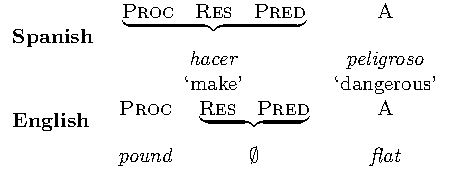
\includegraphics{lexicalization_table}}

Note that this account is consistent with the Borer-Chomsky Conjecture because the variation is lexical in nature.
There is no positive evidence, however, that would allow a learner to determine whether or not the null \textsc{Result} head is present in their linguistic input.
The lack of positive evidence means that this account, while theoretically tenable, predicts that the resultative parameter would be unlearnable.
Therefore, we can reject this analysis.

The final analysis I will address is that of \textcite{kratzer2004building}, which will not be fully reject, but rather adapted to form my final analysis.
In this analysis, the resultative object (\textit{e.g.}, \textit{the metal}) and the adjective (\textit{e.g.}, \textit{flat}) form a small clause, which encodes a state description.
The small clause merges with a \textit{res} head, which encodes a causative relation between events, and the resulting \textit{res}P is merged as the complement of the verb (\textit{e.g.}, \textit{hammer}).
The small clause theme is then raised to check accusative Case, and from there the derivation proceeds as normal.
The structure this generates is given in \Next.
\ex. Kratzer's Resultative Structure\\
{\small
\begin{forest}
  nice empty nodes,sn edges,baseline
  [AgrOP
  [{the metal},name=V theme]
  [
	  [AgrO]
    [VP
	[hammer] 
	[\textit{res}P 
	  [\textit{res}] 
	  [SC
	    [{$\langle\text{the metal}\rangle$},name=sc theme]
	    [flat]
	  ]
	]
      ]
    ]
  ]
  \draw[->] (sc theme) to[out=south west, in=south] (V theme);
\end{forest}}

Under the assumption that \textit{the metal} is $\Theta$-marked by \textit{hammer}, this violates UTAH, and ought to be rejected.
\textcite{kratzer2004building}, however, argues that the objects of resultatives are not $\Theta$-marked by their verbs.
Her arguments against the $\Theta$-marking I assume appear to present problems for me, so I will address them below.

Recall, that my rationale for assuming that the object of a resultative is $\Theta$-marked by its verb was that the entailment in \Next[a] entails \Next[b].
\ex.
\a. Mary hammered the metal flat.
\b. Mary hammered the metal.

In order to argue against this, Kratzer points out that the entailment pattern demonstrated in \Last does not seem to hold of all resultatives.
Specifically, she discusses \Next.
\exg. Die Teekanne leer trinken.\\
The teapot empty drink\\
``Drink the teapot dry/empty.''

In German, as in English, the simple transitive counterpart of \Last is judged odd.
\ex.
\a.? Die Teekanne trinken.
\b.? Drink the teapot.


\subsection{Salvaging parts of previous accounts}
While Snyder's and Kratzer's analyses have been reject, they share a certain feature which I will retain in my final analysis: they are acquirable.
Snyder's (\citeyear{snyder1995language}) proposal is that the availability of resultatives in a language is linked to the availability of a productive N-N compounding in that language.
Kratzer adopts this link and augments it with a link to predicative adjective agreement.
She proposes that resultatives (and N-N compounding) are available only in those languages in which predicative adjectives do not show agreement with the subject.
\ex. \textbf{German}
\ag. Die Teekanne leer trinken.\\
the teapot empty drink.\\
``to dring the teapot dry'' \parencite{kratzer2004building}
\b. Wurmkanne\\
``worm+can'' \parencite{snyder2001nature}
\cg. Die Teekanne ist leer (*-e).\\
The.\textsc{fem} teapot is empty \textsc{fem}''\\
``The teapot is empty.''

\ex. \textbf{Serbo-Croatian} <+Flesh Out These Examples+>

Both compounding and the lack of predicative adjective agreement are detectable in the primary linguistic data, and therefore can reasonably be taken to be the positive data responsible for the setting of the resultative parameter.
The account of the resultative parameter which I will develop in the remainder of this thesis will assume that the positive evidence that triggers the parameter setting will be related to compounding and adjectival agreement.
Before developing such an account, I will modify Kratzer's analysis to make it theoretically feasible in the next chapter.
\end{document}


